


\chapter{Measurement Setup and Calibration }
%\\ \color{green} POST PUBLIC REVIEW VERSION\color{black}}
\label{ch:measurements}
{\color{magenta}{Contributing author: JZ, COM}}{\color{blue}{ -- needs cleanup and some decisions Table \ref{tab:requirements_on_instrumentaion},table \ref{tab:requirements_on_instrumentaion}, section \ref{subsec:selection_of_instrumentation}, section \ref{subsec:measurement-characteristics}, Table \ref{tab:pyranometer_classes}
}}
\color{black}
\noindent
\begin{tcolorbox}
\parbox{\textwidth}{
\emph{\textbf{Key Points}
\begin{itemize}
    \item Instrumentation Selection
                \begin{enumerate}
             \item Evaluation of the required data accuracy or uncertainty levels
            \item Cost-benefit analysis of instrumentation regarding quality and maintenance requirements
            \item Specification on redundancy levels
        \end{enumerate}
    \item Representativeness of Measurements
    \item Verification of correctness of installation and calibration
    \item Setup and Calibration Logging
    \item Maintenance Schedules of instrumentation
\end{itemize}
}}
\end{tcolorbox}

%\section{ TITLE {\color{magenta}{Contributing author: }}}\label{}
%\subsection{TITLE {\color{magenta}{Contributing author: }}}\label{}
\iffalse
\color{red}
Thoughts on this chapter (Corinna):
\begin{itemize}
    \item This is for commenting
    \item balblabla
\end{itemize}

\color{purple}
Changes made by COM: \\
blablabla
\color{black}
\fi

\section{Selection of instrumentation}\label{sec:instrumentation_selection}

{\color{blue}{Comments from SW (28.06.2021: also include comments on how representative the measurements of different instruments are}}

In this section we will describe best practice for the selection of instrumentation for forecasting applications of wind and solar projects. 
We focus in this description not on instruments, but rather on the requirements and necessary considerations for the selection of instrument classes that are appropriate for the pre-defined requirements. 

The first step in the selection procedure is the definition of requirements for the forecasting application. Table \ref{tab:requirements_on_instrumentaion} will provide typical forecasting applications and respective appropriate requirements. 

\begin{longtable}{  p{.20\textwidth} | p{.30\textwidth} |  p{.40\textwidth} }
 \caption{Forecast applications and respective requirements for appropriate instrumentation.}\\
 \hline
 \textbf{Forecast Application} & \textbf{Requirements for Wind} & \textbf{Requirements for Solar}\\ \hline
 \endfirsthead
 \textbf{} & \textbf{} &  \\ \hline
 \endhead
System Operation Forecasting &  Class A & Secondary Standard\\ 
Park control & Class A & Secondary Standard\\ 
Trading & Class B & First Class \\ 
Park Monitoring & Class S & Second Class \\ 
.. & .. & .. \\ 
.. & .. & .. \\ \hline
  \label{tab:requirements_on_instrumentaion}
\end{longtable}

The classes for wind projects are defined in 

\subsection{Selection of instrumentation for wind projects}\label{subsec:instrumentation_selection}

{\color{red}{Comments from COM (21,08,2021):I do not think that this is the goal of our RP here and how the selection of instrumentation should be in our context of real-time forecasting!!!}} \\
\sout{The selection of instrumentation for an operational wind farm should be selected to ensure (1)  its best performance  and (2) reliable power generation. The profitability is connected to the performance of the wind turbines and has to be monitored, as well as each wind turbine and the wind farm in it's entirety needs to be controlled by implementing SCADA systems.}

{\color{green}{Comments from COM (22.08,2021): SUGGESTION\\
The selection of instrumentation of meteorological measurements for forecasting applcations of operational wind farms should be selected to ensure (1) an independent source of measurment to the power generation and (2) a good fit to the power generation of the wind farm. 
}}

In other words, there is a need for appropriate measurement equipment in the sense of: 
\begin{itemize}
    \item Accuracy 
        \begin{itemize}
            \vspace{-0.2cm}\item appropriate quality of instrumentation
           \vspace{-0.2cm} \item uncertainty evaluation of instrumentation
        \end{itemize}
    \item Reliability
        \begin{itemize}
            \vspace{-0.2cm}\item correct installation of instrumentation
           \vspace{-0.2cm} \item correct calibration of instrumentation
            \vspace{-0.2cm}\item redundant setup of instrumentation and logging
        \end{itemize}
    \item Availability
        \begin{itemize}
            \vspace{-0.2cm}\item instruments being redundant
            \vspace{-0.2cm}\item loggers being fail safe
        \end{itemize}
    \item Weather resistant and safe
        \begin{itemize}
            \vspace{-0.2cm}\item meet local requirements of climate
            \vspace{-0.2cm}\item meet local requirements of landscape
            \vspace{-0.2cm}\item meet safety requirements (e.g. flight safe in case of met masts at hub height)
        \end{itemize} 
\end{itemize}


\subsubsection{Components of a wind measurement systems {\color{blue}{Comments from COM (21.08.2021: moved to section \ref{sec:wind_instrumentation}}}}

This list provides a general guidance of the four most important aspects that need consideration in the selection process of instrumentation for real-time forecasting applications. 

It is important for any authority (e.g. TSO, DSO, ultility or balance responsible party) to go through these aspects, when setting requirements for the instrumentation. Dependent on these aspects, there are standards available that guide the wind farm operators to the instrumentation that is appropriate for the requirements set out by the authority. 

In this recommended practice guideline, we therefore focus on the procedure and instrument classes rather than the individual instrumentation, as these are handled by available standards (see section \ref{sec:met_standards} for a description of the applicable standards). 

For wind measurements, there is a principle of three tiers of instrument standard class available that are dependent on the requirements to accuracy and reliability and are also associated with different cost levels. It is therefore recommended to define the requirements first, before requiring a specific instrumentation quality standard. 

The ``GUIDE TO INSTRUMENTS AND METHODS OF OBSERVATION - VOLUME I''\cite{wmoguide2018} defines important requirements for meteorological instruments to:

\begin{enumerate}
    \vspace{-0.2cm}\item Simplicity of design which is consistent with requirements
    \vspace{-0.4cm}\item Durability
    \vspace{-0.4cm}\item Convenience of operation, calibration and maintenance
    \vspace{-0.4cm}\item Acceptable cost of instrument, consumables and spare parts
    \vspace{-0.4cm}\item Safe for staff and the environment
\end{enumerate}

It is recommended that authorities refer to the classification of  instruments in their requirements or provide accuracy limits. 

The IEC 61400 standard \cite{iec61400-12-1-2005}, for example, privides information on anemometers according to class A, class B or class S types, where the classes of instrumentation are dependent on the terrain structure defined in Annex B of the standard. In areas with complex terrain, the class B standard requires e.g. specific setup of instrumentation to accomodate the influence of turbulence from varying terrain etc. 
The class S is associated with specific requirements, ``where  the  influence  parameter  ranges  are  restricted  to  allow  for  the  specified  accuracy  of  the  anemometer.'' \cite{iec61400-12-1-2005}. Manufacturers of wind instrumentation that sell instruments for wind projects provide information about the class of instrumentation to make it easy for wind farm owners to purchase the approapriate instruments. 


The following table describes the main and applicable types of instrument classes in their respective environments. 

\begin{table}[h!]
    \caption{Instrument classes for various environements.{\color{red}{Comments from COM (21.08.2021:NEEDS DISCUSSION and more info}}}
    \centering
    \begin{tabular}{p{4cm}| p{7cm} | p{3cm}}
     \textbf{Environment type}  & \textbf{Environment description} & \textbf{Instrument class} \\ \hline 
     Standard terrain  & Flat terrain with few obstacles & class A \\
     Complex terrain   & varying heights and many obstacles  &  class B\\
     offshore          & wave and current driven turbulence \\ salty air & classe S \\
     ... & & \\
    \end{tabular}
    \label{tab:initial_considerations}
\end{table}



\subsection{Selection of instrumentation for solar power plants}\label{subsec:selection_of_instrumentation}




In the IEA PVPS handbook for the collection and use of solar resource data \cite{nrelhandbook2021} the authors present recommendations for the selection of the instruments. These recommendations also apply for the real-time applications. Depending on the solar technology used different radiation components must be measured. The requirements for fixed monofacial PV or thermal collectors, bifacial PV, concentrating systems and tracked non-concentrating PV are different. Besides radiometers also further meteorological parameters must be measured as stated above. For selecting the instrumentation, the user must also evaluate the required data accuracy and consider the effort necessary to operate and maintain the measurement system. Specifically, the most accurate instrumentation should not be purchased, if the project resources cannot support the maintenance required to ensure measurement quality consistent with the radiometer design specifications and manufacturer recommendations. 
Various radiometers of the same type should be considered for big power plants and are also helpful to ensure a higher data quality. The number of required instruments for PV parks of different peak power is given in IEC 61724-1 along to further requirements on instrument accuracy, maintenance and data logging. Multiple radiometers within a project location and/or providing for the measurement of all three solar irradiance components (GHI, DHI, and DNI) can greatly enhance opportunities for post-measurement data quality assessment.

To summarise, the following considerations should be taken in the selection process:

\begin{enumerate}
    \item Evaluation of the required parameters, data accuracy or uncertainty levels
    \item Cost-benefit analysis of instrumentation regarding quality and maintenance requirements
    \item Specification of number of instruments
\end{enumerate}
   

{\color{red}{Comments from COM (21.08.2021:SUGGESTION --- NEEDS DISCUSSION and ADDED INFORMATION\\

For the selection of pyranometers, the ISO 9060 standard "Solar energy - Specification and classification of instruments for measuring hemispherical solar and direct solar radiation"\cite{ISO9060}, also used and approved by the WMO, separates between 3 classes of instruments. 

\begin{enumerate}
  
    \vspace{-0.2cm}\item Secondary Standard
    \vspace{-0.2cm}\item First Class
    \vspace{-0.2cm}\item Second Class
\end{enumerate}


The following table provides a summary of the applicability of these classes in solar energy forecasting. 
}}
\begin{table}[h!]
    \caption{Pyranometer classes for various requirements. {\color{red}{Comments from COM (21.08.2021:SUGGESTION --- NEEDS DISCUSSION and ADDED INFORMATION}}}
    \centering
    \begin{tabular}{p{6cm} | p{4cm} | p{4cm}}
    \toprule
     \textbf{Requirements}  & \textbf{Instrument class}     & \textbf{Instrument description} \\ \hline 
     Meteorological or Energy forecasting/ modelling &  Secondary Standard & Scientific quality and highest accuracy \\
     & & & \\ 
     Measurements for high level monitoring & First Class & Good quality \\
      & & & \\
     Economic solutions for routine measurements & Second Class & Medium quality \\
     ... & & \\
    \end{tabular}
    \label{tab:pyranometer_classes}
\end{table}


\subsubsection{Components of a PV measurement system}

\subsection{Measurement Characteristics of Different Technologies} \label{subsec:measurement-characteristics}

{\color{magenta}{Discussion of conceptual differences in measurements from anemometers on met masts (point measurements), remote sensing devices (lidar,sodar - which are some type of volume average) and nacelle mounted anemometers (very representative of height and location of turbines but obstructed). \\
}}
{\color{blue}{Questions:\\ Under 4.1.3 (Measurement Characteristics of different technologies), do we want to include solar-related measurements in this?  Ground-based pyranometer vs satellite-based estimate?
}}

\subsubsection{Measurement Characteristics of Lidars}

\textbf{Measuring Laminar Low Level Jets}

An advantage of the remote sensing device's ability to measure the wind profile is it's ability to "measure" low level jets [Kelly et al 2014] that can have significant influence for the power production forecasting. The low level jets are a meteorological phenomenon that is a well-known and extensively researched topic in meteorology since the 1950s [e.g. Blackader, 1957, Zhang, 1996] and has been a topic in wind energy research since forecasting started. 

Recent progress with the help of wind profilers (SODAR, LiDAR) as well as comparisons with a 120m mast has been made in the Lamar Low Level Jet Program, reported by Kelly et al [2014] over a 1-year period. 


\subsubsection{Lightning effects on instrumentation}

It is a know phenomena (e.g. Kelly et al [2014]) that lightning can cause high frequency noise contamination to instruments. 
This is applicable for: 
\begin{itemize}
    \item Remote Sensing instruments (LIDAR, SODAR, RADAR)
    \item sonic anemometers
\end{itemize}

In the case of LIDAR or SODAR lightning contaminates the signal processing with echoes. Such echo reflections can make it impossible for the signal software to process the signal correctly and hence the data cannot be used.
In resource assessment of research projects, such noise can be corrected and the data re-processed to provide valuable data. In Real-time this is not possible. 

In the case of sonic anemometers, high-frequency noise contamination disturbes the sonic signals of wind velocity and temperature and usually makes the data unusable.

\textbf{Maintenance and mitigation methods}
These examples shows that the maintenance and upgrades of software to make use of fixes in the signal processing algorithms of the devices are a key technical requirement for real-time use of the devices, or alternatively that the raw data needs to be sent and the processing takes place where the data is used. 

Therefore, we can conclude that the reliability of any measurement device in real-time operation requires a maintenance schedule to be a technical requirement in order for it not to deteriorate. If this is done, the remote sensing instruments as well as sonic anemometers have proven to provide reliable time series of wind speeds and gusts in general conditions. 





\section{Location of Measurements}\label{sec:location-of-measurements}
        
{\color{magenta}{Comment SW,  COM (21.08.2021): Add an introductory paragraph under 3.1 to describe the issue - that the objective is to make measurements that are well correlated to the power generation (wind or solar) and what issues affect that correlation.}}



{\color{blue}{Comments from John (21.04.2021:\\
Questions: \\
\begin{itemize}
\item Do we know of a guidance that has been written for the horizontal placement of an anemometer or sodar/lidar or solar maesurement for forecasting applications? \\ 
\item  Should the location be well-correlated with the power production from the facility. But what guidance should be provided for that?  \\
Prevailing upstream direction at the roughly the hub height for wind facilities is basic guidance? \\ 
\item  In simple terrain that might be OK but in more complex terrain what guidance can we give?\\
\end{itemize}

More comments from John (JZ) 13.6.2021:

Done: background work on collecting academic papers that have been published on how to determine the most representative \\
 -- location for a single (or two or more..) \\

 --wind measurement(s) to have the highest correlation with the power\\ generation.  
 
 Are there more/any quantitative work that has been done on this?


Intuitive general principles - i.e.\\ 
 (a) place it in the prevailing upstream direction,\\ 
 (b) avoid locations that are frequently in wakes,\\ 
 (c) avoid being near terrain features or roughness elements that are not typical of the overall generation facility etc. 
 
 But can we say more than this? Or show a quantitative example?  Or reference one or more papers?  
 
 What do we say about irradiance measurement location for solar - at the plant centroid? 

Similarly for the vertical location (4.2.2) - measurements near hub height and/or ver

}}







The WMO Report Nr. 55 \cite{wmoreport1993} describes the site and instrumentation selection as a 6-tier problem:
\begin{enumerate}
    \vspace{-0.2cm}\item selection of a suitable site
    \vspace{-0.4cm}\item correct exposure of instruments
    \vspace{-0.4cm}\item determination of the area of representativeness of measurements
    \vspace{-0.4cm}\item description of the site and its facilities
    \vspace{-0.4cm}\item homogeneity of the meteorological/climatological data*
    \vspace{-0.4cm}\item access to information* 
\end{enumerate}

The last two tiers require international collaboration to ensure measured data can be compared and the precision and accuracy of the measured data follows a common understanding for the use in models and methods to improve or interpret model results. We will not deal with these aspects in this document, but want to bring these topics to anyone dealing with measurements to his or her awareness and that the meteorological community has solved these critical problems by establishing international data networks to provide modellers, researchers, instrument developers and end-users the possibility to progress and exchange information. 

The fifth tier deals deals with the lack of international homogeneity on measuring standards that has been a problem in meteorology and can also be observed in wind and solar projects on an international scale. If data measuring standards are not international, it is difficult to obtain homogenity in data and thus models and methods, where such data are used. 


{\color{magenta}{comment SW: I think the following text should be deleted. this belongs to the section "selection of instruments"}\ref{subsec:selection_of_instrumentation}}
\\
{\color{magenta}{One of these problems are the accuracy of instruments. It is very important to define the purpose of measuring and the expectation on the accuracy of the measured quantity. For example, if the accuracy of an instrument is $\mp{0.3}$ and the target is an accuracy of 0.1, neither the instrument nor the measured quantity can provide a representative picture.  }}z







%\subsection{Location of Instrumentation}\label{subsec:selection-of-location}
{\color{magenta}{ Discuss location specifics regarding terrain differences etc.}}
{\color{magenta}{ comment SW 210715: I removed the title "location of instrumentation". I think it is much easier to write and to read if the following text is in the section location of measurements}}
%REPRESENTATIVNESS ???

%\subsection{Measurement Characteristics of Different Technologies}  ---> moved to section 4.1 \ref{subsec:instrumentation_selection}---> search for \ref{subsec:measurement-characteristics}

The Guide for WMO Guide for Meteorological Measurements \cite{guidewmo2018} (``WMO Guide 8'') contains in it's \textit{ANNEX 1.D. SITING CLASSIFICATIONS FOR SURFACE OBSERVING STATIONS ON LAND} information about siting of instrumentation to ensure representativeness. The guide covers all meteorological instrumentation that are relevant for wind and solar projects and operation. 

The WMO Guide 8 states that ``..the environmental conditions of a site may influence measurement results. These conditions must be carefully analysed, in addition to assessing characteristics of the instrument itself, so as to avoid distorting the measurement results and affecting their representativeness..'' and recognises that ``...there are sites that do not respect the recommended exposure rules''. 

Out of these conditions, the WMO has developed a classification with 5 classes to ``help determine the given site’s representativeness on a small scale (impact of the surrounding environment)'' and help to better take their exposure rules into consideration. 

The classes can be summarised to:
\begin{enumerate}
    \vspace{-0.4}\item class: reference site
    \item class: additional uncertainty added by siting through a value relative to the previous class 
    \item class: additional uncertainty added by siting through a value relative to the previous class 
    \item class: additional uncertainty added by siting through a value relative to the previous class 
    \item class: Nearby obstacles create an inappropriate environment for a meteorological measurement that is intended to be representative of a wide area
\end{enumerate}


The most relevant and useful rules to consider also for wind and solar projects are the following:
\begin{itemize}
    \item The classification takes place per instrument, not per site as a whole
    \item The rating of each site should be reviewed periodically as environmental circumstances can change over a period of time
    \item A complete update of the site classes should be done at least every five years
    \item An uncertainty due to siting has to be added in the uncertainty budget of the measurement
    \item The primary objective of the classification should be to document the presence of obstacles close to the measurement site
\end{itemize}


For solar power plants the location of the instruments is of importance as the irradiance can vary within the park due to clouds or shading. Soiling, albedo, wind speed and temperature can also vary strongly. For PV plants recommendations on the number and position of the instruments can be found in IEC 61724-1. Sensors should be distributed over the whole area of the power plant and of course not concentrated at a single site. The location of the instruments should be selected as representative for the covered sections of the power plant. For radiometers mounted on the front side of the PV modules shading should be avoided. For rear side instruments and albedo measurements the number of required radiometers depends also on the variability of the ground surface. For rear side sensors multiple sensors are recommended at different positions on the module, as the illumination profile is not uniform.


\section{Installation of measurement station {\color{blue}{needs attention}}}\label{sec:installation-veification}

{\color{magenta}{comment SW 210715: I removed the word "siting" from the title. This should be all together discussed in the section on instrument location. I commented out the text summarizing the WMO info here as it did seem helpful to me not even for the previous section on location. I assume a general text refering to the CIMO guide will open the section. }}
 
 Specific information on the installation of radiometric stations can be found in \cite{nrelhandbook2021}.
 
%Siting and installation of measurement stations, or ``Automatic Weather Stations'' (\cite{guidewmo2018}) should, according to the WMO Guide \cite{wmoguide2018} be designed so that representative measurements (or observations) can be taken according to the type of station involved. In Meteorology, the distinction is on weather scales such as meso-scale (10-100 km) or synoptic scale ( ~1000km) or aviation observation stations (local). A station in a meso-scale network should make observations to meet meso-scale requirements and an aviation station should describe the conditions specific to the local (aerodrome) site . The WMO Guide further requires that the most stringent requirement will dictate the precise location of an observing site and its associated sensing instruments, where stations are used for several purposes, for example, aviation, synoptic and climatological purposes. A detailed study on siting and exposure is published in WMO (1993).

%%% 

{\color{red}{COM: comment 21.08.2021: I have removed the siting figure from the WMO guide as I think we should not go into this detail, but rather point to the appropriate standards that define everything and rather discuss, what are appropriate reuqirments for real-time forecasting applications}}.

\iffalse
\begin{figure}
    \centering
    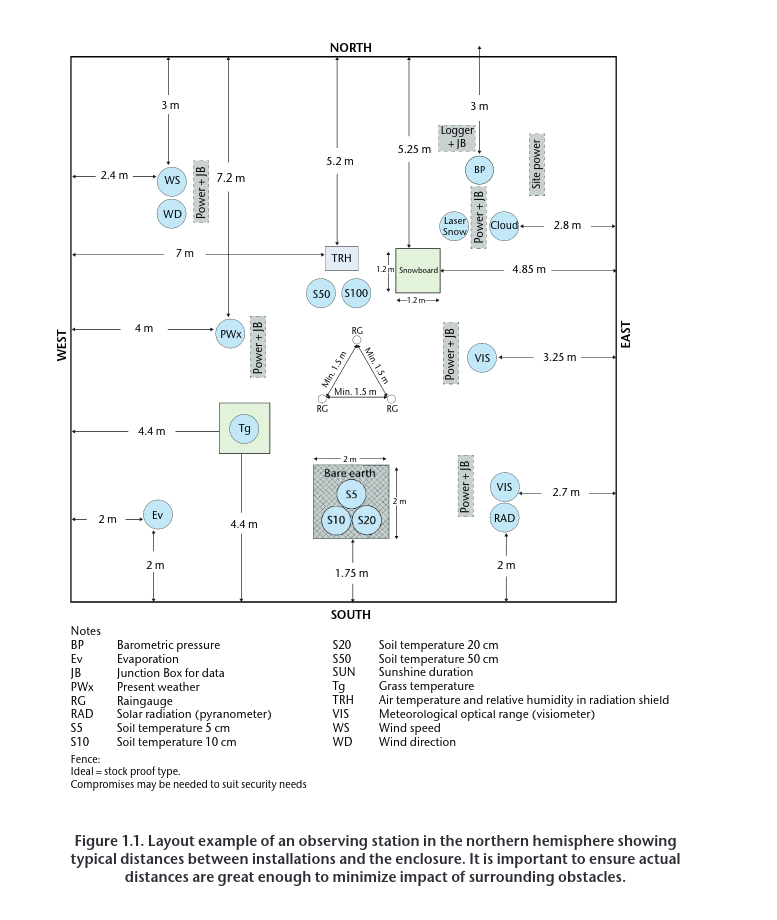
\includegraphics[width=\columnwidth]{figures/screenshots/wmo_nr8_siting.png}
    \caption{Layout example of an observing station in the northern hemisphere showing typical distances between installations and the enclosure . It is important to ensure actual distances are great enough to minimize impact of surrounding obstacles. \copyright WMO Guide to Instruments and Methods of Observation \cite{guidewmo2018}}
    \label{fig:decisionsupporttool}
\end{figure}
\fi

The exposure rules say that...



\subsubsection{Calibration and Correction methodologies for wake effects and yaw misalignment}\label{subsubsec:calibration_and_correctio}

\textbf{Nacelle Anemometers}\\
\cite{Jing2020} for nacelle anemometers
%abstract = {For most wind turbines, blade wakes affect the measurement of nacelle anemometer, result in the inconsistency between nacelle wind speed (NWS) and free stream wind speed, which seriously affects the power forecasting and performance evaluation of wind turbine. This paper proposes a data-driven method to analyse the wake effect on nacelle anemometer. At first, we use Relevance Vector Machine to establish a site calibration model between Lidar wind speed (LWS) and NWS. After that, we can use the calibrated LWS to replace the free stream wind speed, and wake effect on nacelle anemometer can be evaluated by comparing the calibrated LWS and NWS. Then, Wind Turbine Power Curve (WTPC) is applied to make a detail analysis of wake effect on nacelle anemometer. The experimental results show that wake effect accelerates the air velocity behind the impeller. Therefore, WTPC fitted by NWS is “lower” than the real one. However, SCADA system overcorrects the wake effect, thus WTPC fitted by SCADA data is “higher” than the real power curve.}
%This paper proposes a site calibration model based on RVR, it has good performance compared with other typical site calibration methods. Accordingly, we can analyse the wake effect by comparing the LWS and NWS. The experimental results show that when the wind speed exceeds 6 m/s, blade wakes accelerate the air velocity behind the impeller, thus the average value of NWS is about 3\% higher than FSWS for power generation. Due to the wake effect on nacelle anemometer, WTPC fitted by NWS is 8\% “lower” than the real power curve. On the contrary, SCADA system overcorrects the NWS, and WTPC fitted by SWS is about 60\% “higher” than the real one. In the further study, we can use the same method to evaluate the wake effect in higher wind speed range.

\textbf{Scanning Lidars}\\
\cite{Held2019} have developed a method to detect wakes in the inflow of turbines using nacelle lidars and developed a correction method. 
%Nacelle-mounted lidar systems offer the possibility of remotely sensing the inflow of wind turbines. Due to the limitation of line-of-sight measurements and the limited number of focus positions, assumptions are necessary to derive useful inflow characteristics. Typically, horizontally homogeneous inflow is assumed which is well satisfied in flat, homogeneous terrain and over sufficiently large time averages. However, it is violated if a wake impinges the field of view of one of the beams. In such situations, the turbine yaw misalignment measurements show large biases which require the detection and5correction of these observations. Here, a detection algorithm is proposed based on the spectral broadening of the Doppler spectrum due to turbulence within the probe volume. The small-scale turbulence generated within wake flows will typically lead to a significantly larger broadening than in the ambient flow. Thus, by comparing the spectral widths at several locations,situations, where a wake is impinging the field of view of one or more beams can be identified. The correction method is based on an empirical relationship between the difference in turbulence levels at distinct beams and the difference in wind10direction derived from the lidar and the real wind direction. The performance of the algorithm is evaluated in a field experiment identifying all wake situations, and thus, correcting the lidar derived wind direction



 
\section{Maintenance and Inspection Schedules }\label{sec:maintenance-schedules}
The maintenance of the radiometers is often challenging. IEC 61724-1, ASTM G183 and ISO TR9901 recommend maintenance and inspection tasks including
\begin{itemize}
    \vspace{-0.2cm}\item cleaning
    \vspace{-0.4cm}\item levelling/tracking
    \vspace{-0.4cm}\item ventilation 
    \vspace{-0.4cm}\item desiccant
    \vspace{-0.4cm}\item general instrument status incl. cables
    \vspace{-0.4cm}\item and the quality control of the acquired data sets. 
\end{itemize}

    Also the intervals for the different tasks are given. With modern radiometers, and professional installation of the instruments, the task that has to be performed most frequently at the station itself is the cleaning of the sensors. The recommendations for cleaning are between daily (ISO), daily inspection and at least weekly cleaning (ASTM) and weekly cleaning (IEC). In fact the required maintenance frequency depends on the site, the instruments and the accuracy requirement as discussed in \cite{nrelhandbook2021}.  The quality control of the data must also be performed frequently as discussed above. Further information o the maintenance and inspection of solar measurement stations can be found in \cite{nrelhandbook2021}.


%\section{ TITLE {\color{magenta}{Contributing author: }}}\label{}
%\subsection{TITLE {\color{magenta}{Contributing author: }}}\label{}


\subsection{Documentation of setup, calibration, operation}\label{sec:logging-of-calibration}
{\color{blue}{Comment from SW (25.06.2021:  separate subsection seems too much.}}

The United States Environmental Protection Agency (EPA) provides a “Meteorological Monitoring Guidance for Regulatory modelling Applications” \cite{EPA2000} provides recommendations for  reporting for all main meteorological variables used in meteorological modelling.


